\documentclass[main.tex]{subfiles}

\begin{document}

\section{Description of the simulation}

\subsection{Asymmetric Simple Exclusion Process}

The Asymmetric Simple Exclusion Process is a very popular model in statistical physics to model out-of-equilibrium diffusion processes with interacting agents. 
It consists of placing N particles in M boxes, where each box can accommodate a maximum of one particle. 
At a given instant, all particles can jump forward at a certain rate or they can jump backward at a different rate. 
The process is called asymmetric because $\alpha\neq\beta$
However, the simple exclusion means that if the particle is going to jump to a box that is occupied, then the probability is zero.

Under periodic boundary conditions, this process can be solved analytically to show that the particle current (the fraction of particles jumping forward in a given time) depends on the density through the equation 
\begin{gather} j = \qty(\alpha-\beta)\phi\qty(1-\phi)\label{eqn6:current}.\end{gather}
This current goes to zero as the system fills with particles, reminding us of a traffic jam. 

Make a simulation of the ASEP in a periodic system. 
Plot the trajectories of the particles for several densities, and if possible, make an animation. 
Run the simulation many times for each density, find the average current, and plot it against the density. 
Compare it with the analytic result shown above. 

\subsection{Monte Carlo Integration}

Use a Monte-Carlo algorithm to approximate the value of $\pi$. 
Plot the error in this approximation as the number of random samples is increased from 10 to 10e6.

\section{Asymmetric Simple Exclusion Process}\label{sec:asep}

To implement a numerical experiment of the Asymmetric Simple Exclusion Process a modification of the Death and Birth process was done to achieve the the exclusion principle.
First we consider the case in which a particle can move forward or backward,
\begin{gather}
    dN = \left\{
        \begin{array}{ll}
            P(1) &= \alpha dt \\
            P(0) &= 1-\qty(\alpha+\beta) dt \\
            P(-1) &= \beta dt
        \end{array}
    \right.\label{eqn6:case1},
\end{gather}
a second case is when a particle is next to another one and it can only move forwards,
\begin{gather}
    dN = \left\{
        \begin{array}{ll}
            P(1) &= \alpha dt \\
            P(0) &= 1-\alpha dt \\
        \end{array}
    \right.\label{eqn6:case2},
\end{gather}
the third case is similar with the second case, the difference is that instead of going forwards, the particle can only move backwards,
\begin{gather}
    dN = \left\{
        \begin{array}{ll}
            P(0) &= 1-\beta dt \\
            P(-1) &= \beta dt
        \end{array}
    \right.\label{eqn6:case3},
\end{gather}
finally, the fourth case is when the particle is trap between two particles and it can't go forward, neither backwards,
\begin{gather}
    dN = \left\{
        \begin{array}{ll}
            P(0) &= 1
        \end{array}
    \right.\label{eqn6:case4}.
\end{gather}

It is interesting to see that the second and the third case \cref{eqn6:case2,eqn6:case3} are Poisson process with a rate of $\alpha$ and $\beta$, hence, we expect a expected value of $\alpha t$ particles that move forward and $\beta t$ particles that move backward.
On the other hand, the first case \cref{eqn6:case1}, is the Birth and Death process, hence is expected to have $\qty(\alpha-\beta)t$ jumps, which is the overall expected phenomena.

Now, it is important to take into account that the four cases \cref{eqn6:case1,eqn6:case2,eqn6:case3,eqn6:case4}, are descriptions of the movement of one particle and when we add $m$ particles in a discrete space of $M$ spaces, we can analyses the number of jumps done by all the particles  considering how full or empty is the space.

The analytical expression that describes the overall phenomena, \cref{eqn6:current}, was discussed in class.
In the case where we only consider only forward jumps,\cref{eqn6:case2}, the equation \eqref{eqn6:current} is simplify to 
\begin{gather}\alpha\phi\qty(1-\phi)\label{eqn6:jcase2},\end{gather} 
in the case which only backward jumps,\cref{eqn6:case3}, the equation\eqref{eqn6:current} simplifies to
\begin{gather}\beta\phi\qty(1-\phi)\label{eqn6:jcase3}.\end{gather}

\subsection{Numerical results}

In \href{https://github.com/FranVT/NanoTech-Masters/tree/main/1_SisCom/data/data_hk6_4}{this Github repository} there are animation of the numerical implementation of the asymmetric simple exclusion process with packing fractions of \num{0.25},\num{0.5},\num{0.75} and \num{1}.
The number of total boxes is set to 100, hence the maximum of particle is set to 100.
The rate of moving forward and backward was set to $3$ and $2$ respectively, a time differential of \num{1d-2} and \num{500} time steps.
Finally the range of packing fractions was set from $1/80$ to $1$ in steps of $1/80$ and compute 300 simulations for each packing fraction.

\begin{figure}[ht!]
    \centering
    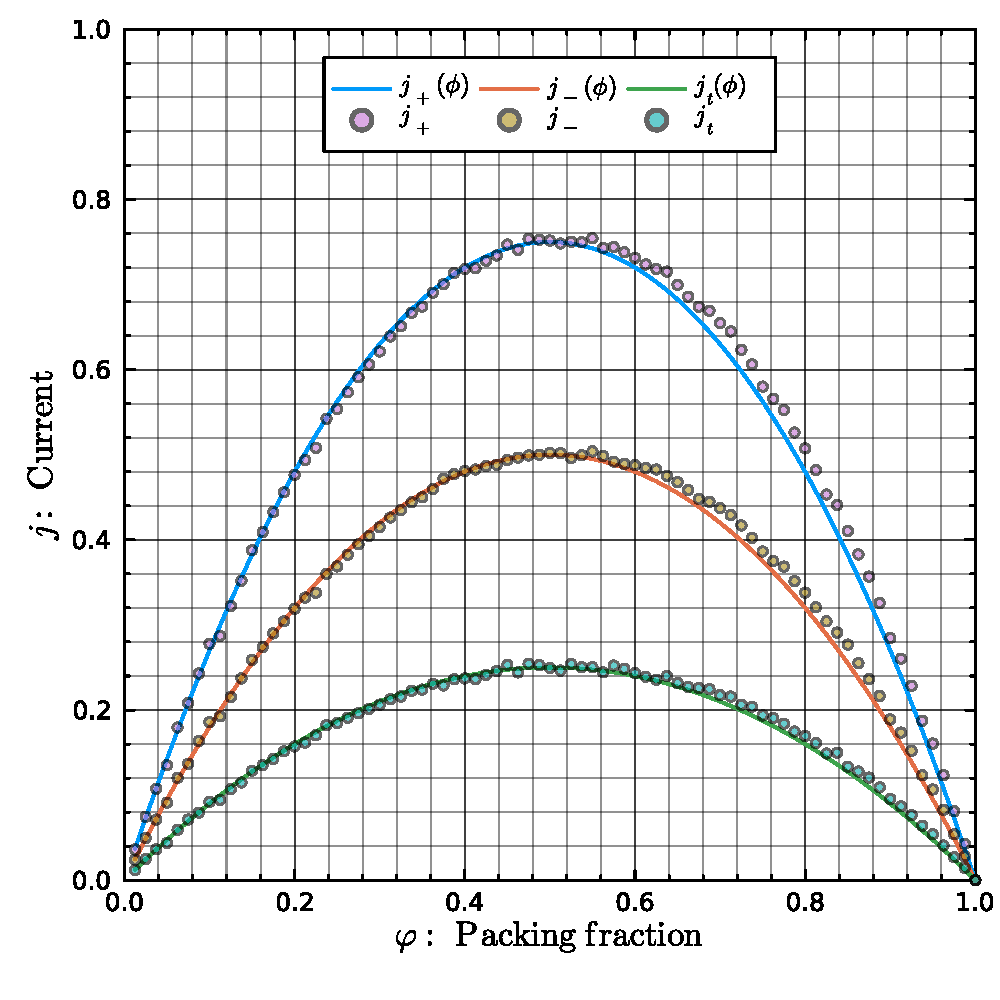
\includegraphics[width=0.8\textwidth]{imgs/hw6/current_packingfraction.pdf}
    \caption{
        Relation between the current with the packing fraction.
        The lines represent the analytical solution and the dots represent the experimental data.
    }
    \label{fig6:asep_jp}
\end{figure}

From each simulation, the number of particles that move forward and backward was re-scaled by the number of total particles in each simulation and store in a file;
The number of total jumps was computed by subtracting the number of total particles that move backwards from the total of particles that move forwards.
Then, the accumulated sum over the time iteration was computed, next the average of all the experiments was computed, finally the last value was store and get the current for each packing fraction.

From that data set, the current in each packing fraction is shown in figure \ref{fig6:asep_jp}.
The continuous lines represent the analytical results given by equations \cref{eqn6:current,eqn6:jcase2,eqn6:jcase3}, represented as $j_t,j_+$ and $j_-$ respectively in the graph, and the experimental values are shown as dots.

Comparing the animations with different packing fraction and the figure \ref{fig6:asep_jp} it can be said that the concept of current is an excellent description of the phenomena, because it shows the effect of adding particles at finite discrete space.
Also, if we realize a thought experiment, when there are few particles, the number of total jumps must be near zero, because there are almost no particles.
When we start adding more particles, the number of jumps must increase, however, by intuition, the number of free spaces to jump decreases, hence there must be a certain number of particles in which makes that the total jumps starts to decreases.
Finally, if we keep adding particles in the finite space, the number of available spaces tends to zero, as the number of total jumps. 

% https://www.sciencedirect.com/science/article/pii/S096007792200443X#f0015
% https://link.springer.com/article/10.1007/s11040-011-9095-1
% https://www.math.ucdavis.edu/~tracy/talks/Stanford2008.pdf
% It is in 2D: https://www.sciencedirect.com/science/article/pii/S0378437117311573

\section{Monte Carlo Integration}

To calculate an estimated value of $\pi$ using a Monte Carlo algorithm, we are going to use the relation of the area of a circle with it radius,
\begin{gather}
    A = \pi r^2.\label{eqn6:areaCricle}
\end{gather}

To calculate the area of a circle using a Monte Carlo algorithm, we set two random with range of $\qty[-0.5,0.5]$, one that represent the values of $x$ and other that represent the values of $y$, then we exclude the values of those random variables such that $x^2+y^2 > 0.5^2$. 
Finally we count all the random numbers which did not exceed the radius and re-escaled the value by normalizing it with respect the number of samples, to get the area of the circle.

Now, that we set an algorithm to get the area, it is important to acknowledge that it set the area of the circle given its diameter, hence \cref{eqn6:areaCricle} is modify,
\begin{gather*}
    A = \pi\qty(\frac{D}{2})^2,
\end{gather*}
then, solving for $\pi$,
\begin{gather}
    \pi = \frac{4}{D^2}A.
\end{gather}

\subsection{Numerical results}

For the numerical implementation, the radius of the circle is set to \num{0.5} and the range of number of samples, for each random variable, is from \num{10} to \num{1d6} with a length of $256$ elements, hence the approximation to the number $\pi$ is,
\begin{gather}
    \pi\approx \frac{4}{N_s}A,
\end{gather}
where $N_s$ is the number of samples used to get the area $A$.

In figure \ref{fig6:relativeErrorMonteCarlo}, it is shown the relative error between the approximation with respect the value of $\pi$ round it at 12 significant digits.
The black dots represent the approximation at $N_s$ samples, and the blue line is just a visual aid.

\begin{figure}[ht!]
    \centering
    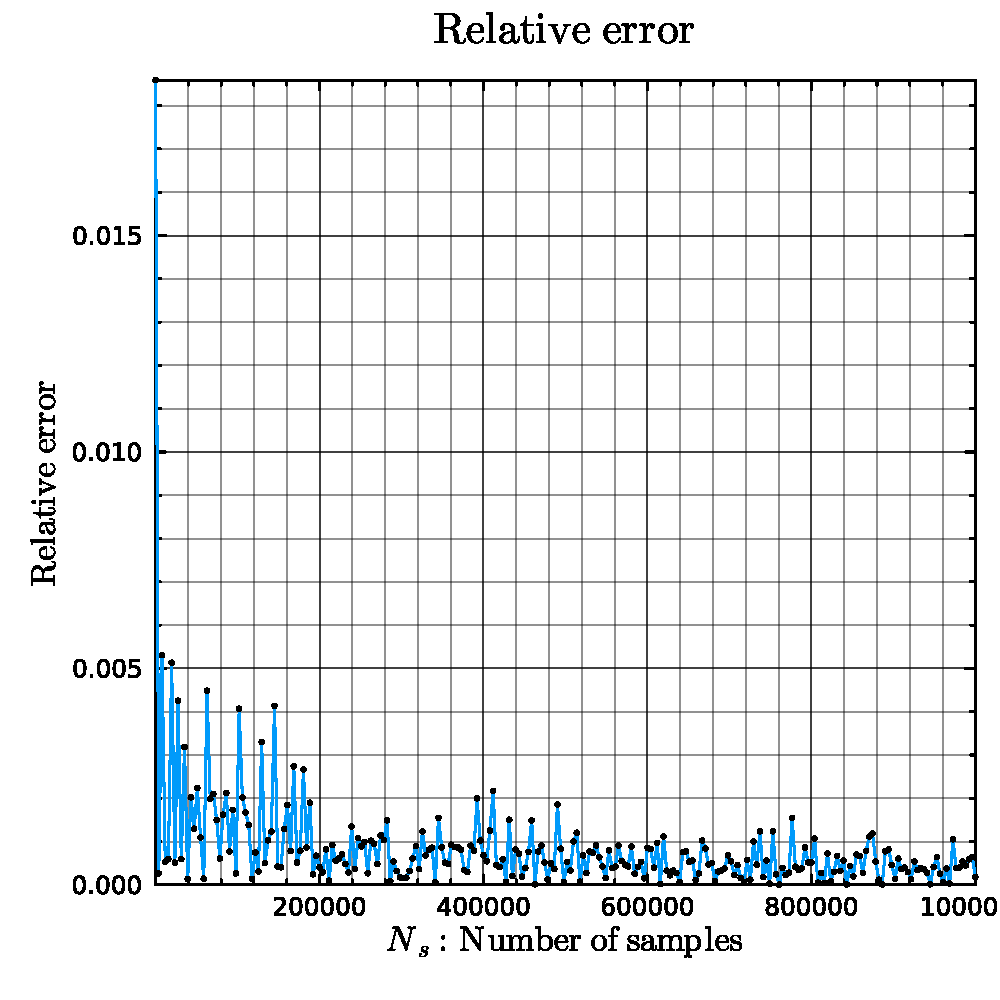
\includegraphics[width=0.8\textwidth]{imgs/hw6/relativeError.pdf}
    \caption{
        Relative error of the approximated value of $\pi$ with 12 significant digits.
    }
    \label{fig6:relativeErrorMonteCarlo}
\end{figure}


% https://discourse.julialang.org/t/speed-up-julia-code-for-simple-monte-carlo-pi-estimation-compared-to-numba/59808
% https://discourse.julialang.org/t/generators-vs-loops-vs-broadcasting-calculate-pi-via-monte-carlo-sampling/63235
    

\end{document}